\documentclass[border=10pt]{standalone}
\usepackage{tikz}
\usetikzlibrary{arrows.meta,positioning,fit,calc}

\begin{document}
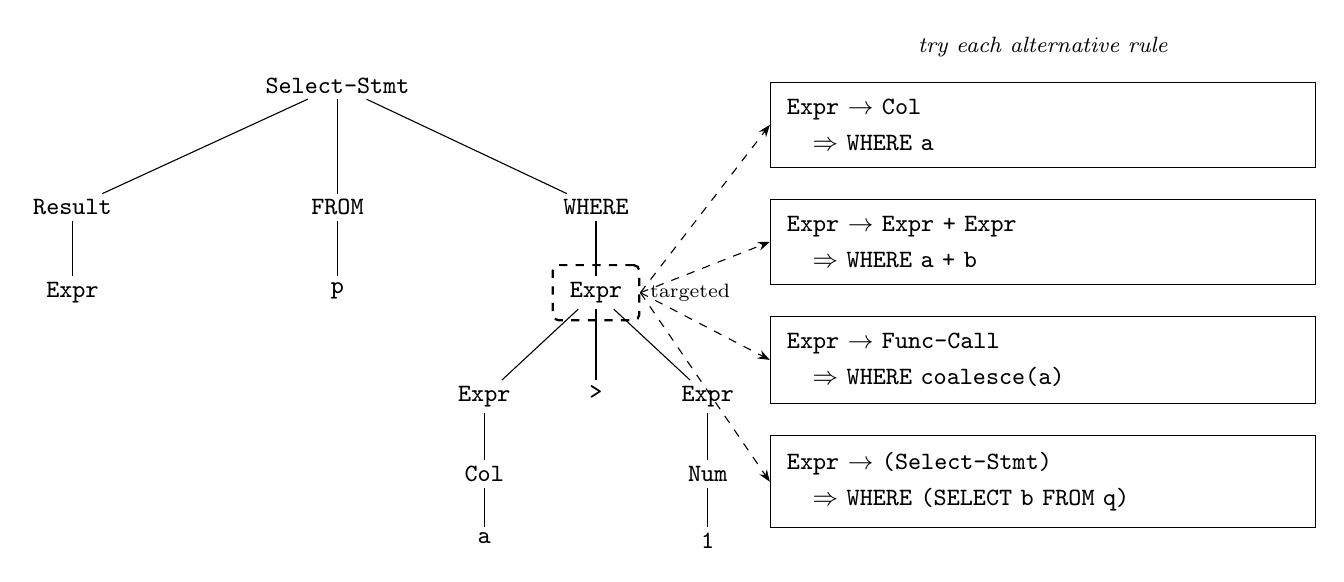
\begin{tikzpicture}[
    every node/.style={font=\small},
    treenode/.style={align=center, inner sep=2pt},
    edge from parent/.style={draw, -{Stealth[scale=0.8]}},
    varbox/.style={rectangle, draw, thin, align=left, inner sep=6pt,
        text width=6.5cm, font=\small},
    dasharrow/.style={-{Stealth[scale=0.9]}, dashed, thin},
]

% ===== LEFT: Input Tree =====
% Root
\node[treenode] (root) {\texttt{Select-Stmt}};

% Level 1
\node[treenode, below left=1.2cm and 1.8cm of root] (result) {\texttt{Result}};
\node[treenode, below=1.2cm of root] (from) {\texttt{FROM}};
\node[treenode, below right=1.2cm and 1.8cm of root] (where) {\texttt{WHERE}};

% Level 2
\node[treenode, below=0.7cm of result] (expr1) {\texttt{Expr}};
\node[treenode, below=0.7cm of from] (p) {\texttt{p}};

% Targeted node with dashed rectangle
\node[treenode, below=0.7cm of where] (target) {\texttt{Expr}};
\node[draw, dashed, thick, rounded corners=2pt, inner sep=4pt, fit=(target),
    label={[font=\scriptsize, anchor=west]right:targeted}] (targetbox) {};

% Level 3 under targeted Expr
\node[treenode, below left=0.9cm and 0.6cm of target] (lexpr) {\texttt{Expr}};
\node[treenode, below=0.9cm of target] (gt) {\texttt{>}};
\node[treenode, below right=0.9cm and 0.6cm of target] (rexpr) {\texttt{Expr}};

% Level 4
\node[treenode, below=0.6cm of lexpr] (col) {\texttt{Col}};
\node[treenode, below=0.6cm of rexpr] (num) {\texttt{Num}};

% Level 5 (leaves)
\node[treenode, below=0.5cm of col] (a) {\texttt{a}};
\node[treenode, below=0.5cm of num] (one) {\texttt{1}};

% Tree edges
\draw (root) -- (result);
\draw (root) -- (from);
\draw (root) -- (where);
\draw (result) -- (expr1);
\draw (from) -- (p);
\draw (where) -- (target);
\draw (target) -- (lexpr);
\draw (target) -- (gt);
\draw (target) -- (rexpr);
\draw (lexpr) -- (col);
\draw (rexpr) -- (num);
\draw (col) -- (a);
\draw (num) -- (one);

% ===== RIGHT: Variant boxes =====
\node[varbox, right=4.5cm of root, yshift=-0.5cm] (v1)
    {\texttt{Expr} $\to$ \texttt{Col}\\[2pt]
     \hspace{1em}$\Rightarrow$ \texttt{WHERE a}};
\node[varbox, below=0.4cm of v1] (v2)
    {\texttt{Expr} $\to$ \texttt{Expr + Expr}\\[2pt]
     \hspace{1em}$\Rightarrow$ \texttt{WHERE a + b}};
\node[varbox, below=0.4cm of v2] (v3)
    {\texttt{Expr} $\to$ \texttt{Func-Call}\\[2pt]
     \hspace{1em}$\Rightarrow$ \texttt{WHERE coalesce(a)}};
\node[varbox, below=0.4cm of v3] (v4)
    {\texttt{Expr} $\to$ \texttt{(Select-Stmt)}\\[2pt]
     \hspace{1em}$\Rightarrow$ \texttt{WHERE (SELECT b FROM q)}};

% Group label
\node[font=\footnotesize\itshape, above=0.2cm of v1] (lbl) {try each alternative rule};

% ===== Dashed arrows from targeted node to variant boxes =====
\draw[dasharrow] (targetbox.east) -- (v1.west);
\draw[dasharrow] (targetbox.east) -- (v2.west);
\draw[dasharrow] (targetbox.east) -- (v3.west);
\draw[dasharrow] (targetbox.east) -- (v4.west);

\end{tikzpicture}
\end{document}
